%%%%%%%%%%%%%%%%%%%%%%%%%%%%%%%%%%%%%%%%%%%%%%%%%%%%%%%%%%%%%%%%%%%%%%%%%%%%%%%%
%2345678901234567890123456789012345678901234567890123456789012345678901234567890
%        1         2         3         4         5         6         7         8

\documentclass[letterpaper, 10 pt, conference]{ieeeconf}  % Comment this line out
                                                          % if you need a4paper
%\documentclass[a4paper, 10pt, conference]{ieeeconf}      % Use this line for a4
                                                          % paper

\IEEEoverridecommandlockouts                              % This command is only
                                                          % needed if you want to
                                                          % use the \thanks command
\overrideIEEEmargins
% See the \addtolength command later in the file to balance the column lengths
% on the last page of the document



% The following packages can be found on http:\\www.ctan.org
\usepackage{graphics} % for pdf, bitmapped graphics files
\usepackage{epsfig} % for postscript graphics files
\usepackage{mathptmx} % assumes new font selection scheme installed
\usepackage{times} % assumes new font selection scheme installed
\usepackage{amsmath} % assumes amsmath package installed
\usepackage{amssymb}  % assumes amsmath package installed
\usepackage{subfigure}

\newcommand{\usequence}[2]{(u_{i,t})_{i=1,t=1}^{#1,#2}}
\newcommand{\contTilde}[1]{\mathbf{\tilde{#1}}}
\newcommand{\transpose}{\mathsf{T}}
\newcommand{\myinner}[1]{\langle(#1)x,x\rangle}
\newcommand{\quadinner}[1]{x^{\transpose}(#1)x}
\DeclareMathOperator{\contB}{\mathbf{B}}
\DeclareMathOperator{\Log}{\mathrm{Log}}
\newcommand{\BK}[1]{\mathbf{B}\bar{K}_{#1}}
%bound \| x_t - x_{t|t} \|
\newcommand{\boundxtxtgt}[2]{C_{fb}^{2}\|\bar{x}_{1}\|[\frac{C_{K}}{\gamma-1}\bigg(\frac{1-(\eta\gamma)^{#1}}{1-\eta\gamma} - \frac{1-\eta^{#1}}{1-\eta} \bigg){#2}+\varepsilon_{K}\bigg(\frac{(#1-1)\eta^{#1+1}-#1\eta^{#1}+\eta}{(1-\eta)^{2}}\bigg)]}
\DeclareMathOperator{\tempRBP}{R + B^{\transpose}PB}

% \newcommand{\boundxtxtgt1}[1]{\frac{#1}{2}}
%bound |K_t|t - K_t^*|
\newcommand{\boundKt}{C_{K^{'}}\gamma^{W-1} + \gamma_{K^{'}}}

%bound xt|t
\newcommand{\boundxtgt}[1]{C_{fb}\eta^{#1}}

% \newcommand{\\det}{\mathit{\det}}
% \newcommand{\Log}[1]{\text{Log}}

\newtheorem{problem}{Problem}
\newtheorem{lemma}{Lemma}
\newtheorem{assumption}{Assumption}
\newtheorem{definition}{Definition}
\newtheorem{corollary}{Corollary}
\newtheorem{proposition}{Proposition}
\newtheorem{remark}{Remark}
\newtheorem{theorem}{Theorem}

\title{\LARGE \bf
Preparation of Papers for IEEE CSS Sponsored Conferences \& Symposia
}

%\author{ \parbox{3 in}{\centering Huibert Kwakernaak*
%         \thanks{*Use the $\backslash$thanks command to put information here}\\
%         Faculty of Electrical Engineering, Mathematics and Computer Science\\
%         University of Twente\\
%         7500 AE Enschede, The Netherlands\\
%         {\tt\small h.kwakernaak@autsubmit.com}}
%         \hspace*{ 0.5 in}
%         \parbox{3 in}{ \centering Pradeep Misra**
%         \thanks{**The footnote marks may be inserted manually}\\
%        Department of Electrical Engineering \\
%         Wright State University\\
%         Dayton, OH 45435, USA\\
%         {\tt\small pmisra@cs.wright.edu}}
%}

\author{Yitian Chen, Timothy Molloy, Iman Shames% <-this % stops a space
% \thanks{This work was not supported by any organization}% <-this % stops a space
% \thanks{H. Kwakernaak is with Faculty of Electrical Engineering, Mathematics and Computer Science,
%         University of Twente, 7500 AE Enschede, The Netherlands
%         {\tt\small h.kwakernaak@autsubmit.com}}%
% \thanks{P. Misra is with the Department of Electrical Engineering, Wright State University,
%         Dayton, OH 45435, USA
%         {\tt\small pmisra@cs.wright.edu}}%
}


\begin{document}



\maketitle
\thispagestyle{empty}
\pagestyle{empty}


%%%%%%%%%%%%%%%%%%%%%%%%%%%%%%%%%%%%%%%%%%%%%%%%%%%%%%%%%%%%%%%%%%%%%%%%%%%%%%%%
\begin{abstract}

\end{abstract}


%%%%%%%%%%%%%%%%%%%%%%%%%%%%%%%%%%%%%%%%%%%%%%%%%%%%%%%%%%%%%%%%%%%%%%%%%%%%%%%%
\section{INTRODUCTION}
Consider the linear systems
\begin{align}
    &x_{t+1} = Ax_{t} + \mathbf{B}\mathbf{u}_{t}\label{eq:linsys},\\
    &x_{1} =\bar{x}_{1}(\bar{x}_1 \in \mathbb{R}^{n})\label{eq:initialx}
\end{align}
where $t$ is an nonegative integer, $m$ and $n$ are positive integers, $A \in \mathbb{R}^{n\times n}$, $\mathbf{B} := [B^{1}, B^{2}]$, $B^{i} \in \mathbb{R}^{n\times m}(1\leq i \leq 2)$, $\mathbf{u}_{t} = [u_{1,t}^{\transpose},u_{2,t}^{\transpose}]^{\transpose}$, $x_{t}\in\mathbb{R}^n$ and $u_{i,t} \in \mathbb{R}^{m}$($1\leq t \leq T,1\leq i \leq 2$). 
Given $\mathbf{H}$ with 2 rows partitions and 2 column partitions, i.e.,
\begin{align*}
    \mathbf{H} = 
    \begin{bmatrix}
        H_{11} & H_{12}\\
        H_{21} & H_{22}
    \end{bmatrix}.
\end{align*}
For each $i,j(1\leq i,j\leq 2)$, we define the notation
\begin{equation}
    [\mathbf{H}]_{ij} := H_{ij}.
\end{equation}


Moreover, define the following notations
\begin{align}
    &(u_{i,t})_{i=1,t=1}^{2,T-1} := (u_{1,1},u_{2,1},\cdots, u_{1,T-1},u_{2,T-1}),\\
    \begin{split}
         &(u_{i,t})_{i=1,t=1}^{2,\tau-1} \frown (v_{i,t})_{i=1,t=\tau}^{2,T-1}:=(u_{1,1},\cdots,u_{1,\tau-1},v_{1,\tau},\cdots,\\
    &\qquad v_{1,T-1},u_{2,1},\cdots,u_{2,\tau-1},v_{2,\tau},\cdots,v_{2,T-1} ),
    \end{split}
   \\ 
   & R_{t}^{i} := 
   \begin{bmatrix}
       [R_{t}^{i}]_{11} & [R_{t}^{i}]_{12}\\
       [R_{t}^{i}]_{21} & [R_{t}^{i}]_{22}
   \end{bmatrix}(1\leq i \leq 2),\\
    &g_{i,t}(x_{t}, \mathbf{u}_{t}) := \frac{1}{2}(x_{t}^{\mathsf{T}}Q_{t}^{i}x_{t} + 
    \mathbf{u}_{t}^{\transpose}R_{t}^{i}\mathbf{u}_{t})(1\leq i \leq 2),\\
    &g_{i,T}(x) := \frac{1}{2} x^{\mathsf{T}}Q_{T}^{i}x(1\leq i \leq 2).
\end{align}
For all $1 \leq t \leq T$ and $1\leq i\leq 2$, the matrices $Q_{t}^{i}$, $[R_{t}^{i}]_{pq}(1\leq p,q \leq 2)$, $A$ and $B^{i}(1\leq i \leq 2)$ satisfy the following assumptions
\begin{assumption}\label{assumption:bounds}
    There exists symmetric positive definite matrices $Q_{min}, Q_{max}, R_{min}, R_{max}$ that
    \begin{equation}
        Q_{min} \preceq Q_{t} \preceq Q_{max},
    \end{equation}
    \begin{equation}
        Q_{t} \in \mathbb{S}^{n}_{++},
    \end{equation}
    for $1\leq t \leq T$, and
    \begin{equation}\label{eq:positiveR}
        R_{min} \preceq 
        \begin{bmatrix}
            [R_{t}^{1}]_{11} & [R_{t}^{1}]_{12}\\
            [R_{t}^{2}]_{21} & [R_{t}^{2}]_{22}
        \end{bmatrix}
        \preceq R_{max},
    \end{equation}
    for $1 \leq t \leq T-1$.
\end{assumption}
\begin{assumption}\label{assumption:controllable}
    Matrix $A$ has full rank, and there exists $\bar{K}$, such that $\rho(A + \contB \bar{K}) < 1$, where $\rho(\cdot)$ denotes the spectral radius operator.
\end{assumption}
Define the cost function for the $i$-th player,
\begin{equation}\label{eq:LQcost}
    J_{i,T}((x_{t})_{t=1}^{T},(u_{i,t})_{i=1,t=1}^{N,T-1}) := \sum_{t=1}^{T-1} g_{i,t}(x_{t}, \mathbf{u}_{t}) + g_{i,T}(x_{T}).
\end{equation}

Before we start discussing feedback Nash equilibrium, we use $(u_{i,t}^{*})_{i=1,t=1}^{2,T-1}$ to denote the control sequence for feedback Nash equilibrium, and $(u_{i,t})_{i=1,t=1}^{2,T-1}$ is a sequence that consisted by any given control vectors for each player. 

Furthermore, for $1 \leq \tau \leq T$, $(x_{t}^{*\tau})_{t=1}^{T}$ is generated by the sequence of $(u_{i,t})_{i=1,t=1}^{2,\tau-1} \frown (u_{i,t}^{*})_{i=1,t=\tau}^{2,T}$, where $u_{i,t}$ is any given control decision for $1 \leq i \leq 2$ and $1 \leq t \leq \tau-1$. Moreover, for $1 \leq \tau \leq T$, $(x_{t}^{(1,\tau)})_{t=1}^{T}$ is generated by $(u_{i,t})_{i=1,t=1}^{2,\tau-1} \frown (u_{1,\tau},u_{2,\tau}^{*}) \frown (u_{i,t}^{*})_{i=1,t=\tau+2}^{2,T}$. Similarly to $(x_{t}^{(2,\tau)})_{t=1}^{T}$.

The sequence $( u_{i,t}^{*})_{i=1,t=1}^{2,T}$ satisfies that, for any fix $i$ that $1 \leq i \leq 2$, such 
sequence satisfies that 
\begin{equation}\label{eq:nashIneq}
    \begin{split}
        \text{Level T}
        &\begin{cases}
            &J_{1,T}((x_{t}^{*T})_{t=1}^{T}, (u_{i,t})_{i=1,t=1}^{2,T-2} \frown (u_{1,T}^{*},u_{2,T}^{*})) \\ & \leq J_{1,T}((x_{t}^{(1,T)})_{t=1}^{T}, (u_{i,t})_{i=1,t=1}^{2,T-2} \frown (u_{1,T},u_{2,T}^{*})),\\ \\
            &J_{2,T}((x_{t}^{*T})_{t=1}^{T}, (u_{i,t})_{i=1,t=1}^{2,T-2} \frown (u_{1,T}^{*},u_{2,T}^{*})) \\ & \leq J_{2,T}((x_{t}^{(2,T)})_{t=1}^{T}, (u_{i,t})_{i=1,t=1}^{2,T-2} \frown (u_{1,T}^{*},u_{2,T})).
        \end{cases}
    \\ &\qquad \qquad \qquad \vdots \\
    \text{Level 1}
        &\begin{cases}
            &J_{1,T}((x_{t}^{*1})_{t=1}^{T}, (u_{1,1}^{*},u_{2,1}^{*}) \frown (u_{i,t}^{*})_{i=1,t=2}^{2,T-1}) \\ & \leq J_{1,T}((x_{t}^{(1,1)})_{t=1}^{T}, (u_{1,1},u_{2,1}^{*}) \frown (u_{i,t}^{*})_{i=1,t=2}^{2,T-1}),\\ \\
            &J_{2,T}((x_{t}^{*1})_{t=1}^{T}, (u_{1,1}^{*},u_{2,1}^{*}) \frown (u_{i,t}^{*})_{i=1,t=2}^{2,T-1}) \\ & \leq J_{2,T}((x_{t}^{(2,1)})_{t=1}^{T}, (u_{1,1}^{*},u_{2,1}) \frown (u_{i,t}^{*})_{i=1,t=2}^{2,T-1}).
        \end{cases}
    \end{split}
\end{equation}

For convenient use later, we define the notion of $\mathcal{H}_{t}$ and $\text{DFLGame}$ as
\begin{equation}\label{eq:history}
    \mathcal{H}_{T} := ( \bar{x}_{1},(Q_{t}^{i})_{i=1,t=1}^{2,T},(R_{t}^{i})_{i=1,t=1}^{2,T-1}),
\end{equation}
\begin{equation}\label{eq:regret}
 \text{DFLGame}(\mathcal{H}_{T},T):=((x_{t}^{*1})_{t=1}^{T}, (\mathbf{u}_{t}^{*})_{t=1}^{T-1}).
\end{equation}
% and the problem of finding such $(x_{t}^{*1})_{t=1}^{T}, (u_{i,t}^{*})_{i=1,t=1}^{2,T-1}$ is called a linear quadratic dynamic feedback game(LQDFG).
For any decisions $(\mathbf{u}_{t})_{t=1}^{T-1}$ and the associated state sequence $(x_{t})_{t=1}^{T}$, the dynamic social regret is defined as
\begin{equation}
    \begin{split}
        &\text{Regret}_{T}((\mathbf{u}_{t})_{t=1}^{T-1}) := \\
        &\sum_{i=1}^{N} J_{i,T}((x_{t})_{t=1}^{T},(\mathbf{u}_{t})_{t=1}^{T-1}) - J_{i,T}((x_{t}^{*})_{t=1}^{T},(\mathbf{u}_{t}^{*})_{t=1}^{T-1}).
    \end{split}
\end{equation}
The main focus of our work is to propose a novel control policy that generates $\mathbf{u}_{t}$ using the information available at time $t$, i.e., $\mathcal{H}_{t}$, and investigate its performance. We specifically consider a feedback control policy $\pi(\cdot,\cdot)$ of the form 
\begin{equation}\label{eq:policyForm}
    \mathbf{u}_{t} = \pi(x_{t}, \mathcal{H}_{t}).
\end{equation}

The key contributions of this paper are
\begin{itemize}
    \item The proposal of a method to solve an online LQ potential game;
    \item Development of the dynamic social regret upperbound;
\end{itemize}



%%%%%%%%%%%%%%%%%%%%%%%%%%%%%%%%%%%%%%%%%%%%%%%%%%%%%%%%%%%%%%%%%%%%%%%%%%%%%%%%
\section{PROBLEM FORMULATION}
In this paper, we consider the following problem.
\begin{problem}[Online Dynamic LQ Game]
     Consider the system \eqref{eq:linsys}. Let the cost matrices in \eqref{eq:regret} satisfy Assumption \ref{assumption:controllable} for any given $T \geq 1$ and $W < T-1$. At time $1 \leq t \leq T-W-1$, the available information to the players is given by $\mathcal{H}_{t}$ as defined in \eqref{eq:history} and the current state $x_{t}$. It is desired to design a control policies $\pi(\cdot, \cdot)$ of the form \eqref{eq:policyForm} that yields a regret, as defined by \eqref{eq:regret}, ???.
     % , that is independent of the bounds given in Assumption \ref{assumption:bounds}.
\end{problem}

\section{APPROACH AND REGRET ANALYSIS}
\paragraph{Prediction. } 
Define 
\begin{equation}
\begin{split}
    \bar{\mathcal{H}}_{t} = (&\bar{x}_{1}, (Q_{\tau})_{\tau=1}^{t+W} \frown(Q_{t+W})_{\tau=t+W+1}^{T},\\
    &(R_{\tau}^{i})_{i=1,\tau=1}^{2,t+W} \frown(R_{t+W}^{i})_{i=1,\tau=t+W+1}^{2,T-1}).
\end{split}
\end{equation}
We predict a trajectory by using the current cost matrices and setting the future unknown cost matrices to be equal to the known value at time $t+W$, i.e.,
\begin{equation}
    ((x_{\tau|t})_{\tau=1}^{T},(\mathbf{u}_{\tau|t})_{\tau=1}^{T-1}) = \text{DFLGame}(\bar{\mathcal{H}}_{t},T).
\end{equation}

\paragraph{Prediction Tracking. } We propose the following feedback control policy
\begin{equation}\label{eq:policy}
    \pi(x_{t},\mathcal{H}_{t}) := \bar{K}(x_{t}-x_{t|t}) + \mathbf{u}_{t|t},
\end{equation}
where $\bar{K}\in \mathbb{R}^{m\times n}$ is a control matrix such that $\rho(A+\mathbf{B}\bar{K}) < 1$, and $\rho(\cdot)$ denotes the matrix spectral radius.


\subsection{Regret Analysis}
Consider the linear system defined by \eqref{eq:linsys}. For a given time horizon $T \geq 1$ and preview window length $0 \leq W \leq T-1$. Suppose that at time $1\leq t \leq T-1$ the control input $u_{t}$ is generated by $\pi(\cdot,\cdot)$ as given by \eqref{eq:policyForm}. Under Assumption \ref{assumption:bounds},\ref{assumption:controllable},\ref{ass}
\begin{definition}[LQDFG]\label{def:LQDFG}
    A linear quadratic dynamic feedback game(LQDFG) is, for each player $i(1\leq i\leq 2)$ and a given positive integer $T$, suppose $J_{i,t}(\cdot,\cdot)$ for $1\leq i\leq 2,1\leq t\leq T$ are known by each player, where $J_{i,t}$ is defined at \eqref{eq:LQcost}. At stage $t(1\leq t\leq T-1)$, each player chooses the control $u_{i,t}^{*}$ that satisfies the inequalities given in \eqref{eq:nashIneq}. 
\end{definition}

% Before we introduce the concept of linear quadratic dynamic feedback potential game(LQDFPG), let's start by introducing the following linear quadratic optimal control problem(LQOCP). For a given $T(T\geq 1)$, 
% suppose $\Psi_{t}:\mathbb{R}^{n}\times\mathbb{R}^{m}\rightarrow \mathbb{R}(1\leq t \leq T-1)$ and $\Psi_{T}:\mathbb{R}^{n}\rightarrow \mathbb{R}$ are being continuous and twice continuously differentiable in their arguments.
Under Assumption \ref{assumption:controllable}, LQOCP is defined by the following problem.

\begin{definition}[LQOCP]\label{def:LQOCP}
    The problem of linear quadratic optimal control problem(LQOCP) is the following.
    Suppose $T$ is a positive integer. For given $(\bar{Q}_{t})_{t=1}^{T},(\bar{R}_{t})_{t=1}^{T-1}$ satisfy (...existence of solution), find $\{\mathbf{u}_{t}\}_{t=1}^{T-1}$ such that
    \begin{equation}\label{eq:LQOCP}
\begin{split}
    \min_{\{\mathbf{u}_{t}\}_{t=1}^{T-1}}& \sum_{t=1}^{T-1} x_{t}^{\transpose}\bar{Q}_{t}x_{t} + \mathbf{u}_{t}^{\transpose}\bar{R}_{t}\mathbf{u}_{t} + x_{T}^{\transpose}\bar{Q}_{T}x_{T}\\
    &\text{\qquad subject to Equation \eqref{eq:linsys}}.
\end{split}
\end{equation}
\end{definition}



\begin{definition}
    The dynamic game is referred to as a linear quadratic dynamic feedback potential game(LQDFPG), if the solution of a given LQOCP, in feedback form, provides a feedback Nash equilibrium for the linear quadratic dynamic game. 
\end{definition}

\begin{lemma}
    For time instant $t$ from $T-1$ to 1, define
        \begin{equation}\label{eq:Theta}
        [\Theta_{t}]_{ij} := [R_{t}]^{i}_{ij} + B^{i\transpose}P_{t+1}^{i}B^{j},
        \end{equation}
    where $R_{t}^{1},R_{t}^{2},Q_{t}$ from a LQDFG satisfy
        \begin{equation}\label{eq:costFPDG1}
            [R_{t}^{1}]_{12} + B^{1\transpose}P_{t+1}^{1}B^{2} = ([R_{t}^{2}]_{21} + B^{2\transpose}P_{t+1}^{2}B^{1})^{\transpose}(1\leq t\leq T-1),
        \end{equation}
        \begin{equation}\label{eq:costFPDG2}
            \Theta_{t} \succ 0(1\leq t \leq T-1),
        \end{equation}
        \begin{equation}\label{eq:costFPDG3}
            \mathbf{B}^{\transpose}(P_{t}^{1}-P_{t}^{2})A=0(1\leq t \leq T),
        \end{equation}
    Then, the LQDFG that has such parameters is a linear quadratic dynamic feedback potential game(LQDFPG).
\end{lemma}
The above lemma is a special case of \cite[Theorem 6]{prasad_structure_2023} when $Q_{t}^{1}=Q_{t}^{2}$ for $t(1\leq t \leq T)$.

\begin{lemma}\label{lemma:gamePGrelation}
    Consider an LQDFPG and LQOCP described by \ref{def:LQDFG} and \ref{def:LQOCP} respectively. Let Assumptions \ref{assumption:bounds} hold. Further, consider the relationships
    \begin{align*}
        &\bar{P}_{T} = \bar{Q}_{T},\\
        &\bar{\Theta}_{t} = \bar{R}_{t} + \contB^{\transpose}\bar{P}_{t+1}\contB,\\
        &\bar{K}_{t} = \bar{\Theta}_{t}^{-1}\contB^{\transpose}\bar{P}_{t+1}A,\\
        &\bar{P}_{t} = \bar{Q}_{t} + \bar{K}_{t}^{\transpose}\bar{R}_{t}\bar{K}_{t} + (A+\contB\bar{K}_{t})^{\transpose}\bar{P}_{t+1}(A+\contB\bar{K}_{t}),
    \end{align*}
    for $(1\leq t \leq T-1)$,
    and
    \begin{align*}
        \bar{\Theta}_{t} \succ 0,
    \end{align*}
    hold.
    Assume that the following relation is satisfied,
    \begin{equation}
        [R_{t}^{i}]_{ii} + B^{i\transpose}P_{t+1}^{i}B^{i} = [\bar{R}_{t}]_{ii} + B^{i\transpose}\bar{P}_{t+1}B^{i},
    \end{equation}
    \begin{equation}
        B^{i\transpose}P_{t+1}^{i}A = B^{i\transpose}\bar{P}_{t+1}A,
    \end{equation}
    \begin{equation}
        [R_{t}^{i}]_{ij} + B^{i\transpose}P_{t+1}^{i}B^{j} = [\bar{R}_{t}]_{ij} + B^{i\transpose}\bar{P}_{t+1}B^{j},i\neq j,
    \end{equation}
    \begin{equation}
        [R_{t}^{1}]_{12} + B^{1\transpose}P_{t+1}^{1}B^{2} = ([R^{2}_{t}]_{21} + B^{2\transpose}P^{2}_{t+1}B^{1})^{\transpose},
    \end{equation}
    for $i,j=1,2$ and $1\leq t \leq T-1$. Then, the LQDFPG defined in Definition \ref{def:LQDFG} is associated with the LQOCP defined in Definition \ref{def:LQOCP}.
\end{lemma}


\begin{lemma}
    \cite[Theorem 5]{prasad_structure_2023}
    For a given positive integer $T$, define
    \begin{align*}
        \Omega := ((\bar{Q}_{1},\bar{Q}_{2},\cdots,\bar{Q}_{T},\bar{R}_{1},\cdots,\bar{R}_{T-1})|\mathcal{K}),
    \end{align*}
    where $\mathcal{K}$ is the conditions that, at time instant $T$, $\bar{Q}_{T}$ is such that
        \begin{equation}
            \mathbf{B}^{\transpose}\bar{Q}_{T}A = \mathbf{B}^{\transpose}Q_{T}A,
        \end{equation}
        and, let $\bar{P}_{T}$ satisfy
        \begin{equation}
            \mathbf{B}^{\transpose}\bar{P}_{T}A = \mathbf{B}^{\transpose}Q_{T}A.
        \end{equation}
        Moreover, set $\bar{R}_{t}$ as
        \begin{equation}\label{eq:matrixR}
            \bar{R}_{t} = \Theta_{t} - \mathbf{B}^{\transpose}\bar{P}_{t+1}\mathbf{B},
        \end{equation}
        where $\Theta_{t} \succ 0$,
        with $\bar{Q}_{t}$ such that
        \begin{equation}
            \bar{Q}_{t} = Q_{t} + K_{t}^{\transpose}(R_{t}^{1}-\bar{R}_{t})K_{t},
        \end{equation}
        where
        \begin{equation}
            K_{t} = \Theta_{t}^{-1}
            \begin{bmatrix}
                B_{t}^{1\transpose}P_{t+1}^{1}\\
                B_{t}^{2\transpose}P_{t+1}^{2}
            \end{bmatrix}
            A,
        \end{equation}
        from $t=T-1$ to $t=1$.
    Then, every element in $\Omega$ is an associated LQOCP for the LQDFPG. Further, $\Omega$ is non-empty.
\end{lemma}
\begin{assumption}\label{assumption:lowerQ}
    For any given $t(1\leq t \leq T-1)$, matrices $Q_{t}, R_{t}^{1}, \bar{R}_{t}$ satisfy
    \begin{equation}
        \lambda_{\min}(Q_{t}) > \max(0,\sigma_{max}(B)\lambda_{min}(\bar{R}_{t}-R_{t}^{1}))
    \end{equation}
\end{assumption}
\begin{assumption}\label{assumption:DGparameters}
    An LQDFG with parameters $\{Q_{\tau|t}\}_{\tau=1}^{T}$ and $\{R_{\tau|t}\}_{\tau=1}^{T-1}$ is an LQDFPG.
\end{assumption}
\begin{lemma}\label{lemma:boundedP}
    Define
    \begin{equation}
        \bar{P}_{T} = \bar{Q}_{T},
    \end{equation}
    for $t = T$, and 
    \begin{equation}
    \begin{split}
        &\bar{K}_{t} = -(R_{t}+ B^{\transpose}\bar{P}_{t+1}B)^{-1}B^{\transpose}\bar{P}_{t+1},\\
        &\bar{P}_{t} = \bar{Q}_{t} + \bar{K}_{t}^{\transpose}\bar{R}_{t}\bar{K}_{t} + (A+B\bar{K}_{t})^{\transpose}\bar{P}_{t+1}(A+B\bar{K}_{t}),
    \end{split}
    \end{equation}
    for $1\leq t \leq T-1$, recursively. There exists positive definite matrices $\bar{P}_{min}$ and $\bar{P}_{max}$ such that
    \begin{equation}
        0 \prec \bar{P}_{min} \preceq \bar{P}_{t} \preceq \bar{P}_{max}.
    \end{equation}
\end{lemma}
\begin{theorem}
Consider the linear system defined by \eqref{eq:linsys}. For a given time horizon $T \geq 1$ and preview window length $0 \leq W \leq T-1$. Suppose that at time $1 \leq t \leq T-1$ the control input $u_t$ is generated by policy $\pi(\cdot,\cdot)$ as given by \eqref{eq:policyForm}. Under Assumption \ref{assumption:bounds}-\ref{assumption:DGparameters}, the regret defined by \eqref{eq:regret} satisfies
    \begin{align*}
        \text{Regret}_{T}((\mathbf{u}_{t})_{t=1}^{T-1})
        \leq \|\bar{x}_{1}\|^{2}\bigg[&\Delta_{a}\frac{1-q^{2T}}{1-q^{2}} + \Delta_{b}(\gamma^{W},\varepsilon_{K^{'}})\frac{1-\eta^{2T}}{1-\eta^{2}}\\
        &+ \Delta_{c}(\gamma^{W},\varepsilon_{K^{'}})\frac{1-(q\eta)^{T}}{1-q\eta}\bigg],
    \end{align*}
    where 
\end{theorem}



%%%%%%%%%%%%%%%%%%%%%%%%%%%%%%%%%%%%%%%%%%%%%%%%%%%%%%%%%%%%%%%%%%%%%%%%%%%%%%%%
\section{NUMERICAL SIMULATIONS}
\begin{figure}
        \label{fig:different_cases}
     \centering
     \subfigure[Regret vs. Time Horizon with 0 Preview Window Length]{
         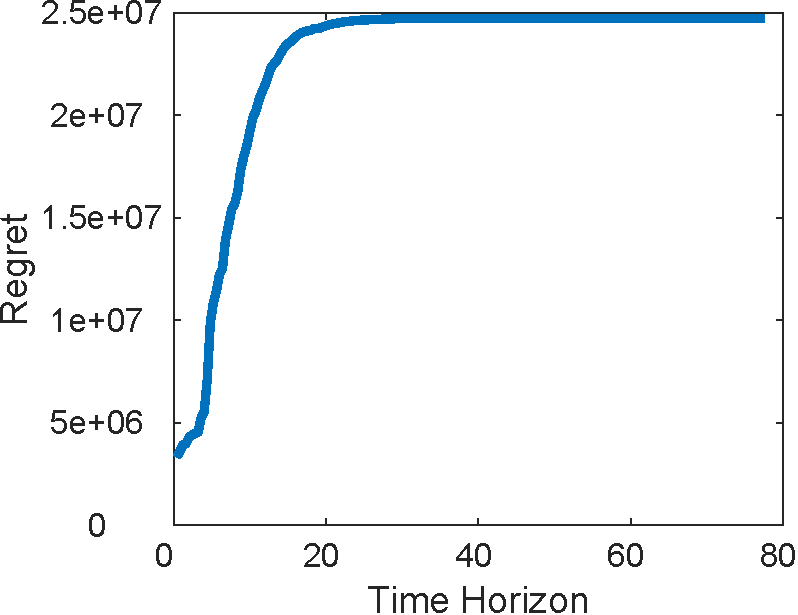
\includegraphics[width=.3\textwidth]{window1.pdf}
    \label{fig:physSysReg}}
     \subfigure[Regret vs. Time Horizon with 1 Preview Window Length]{
         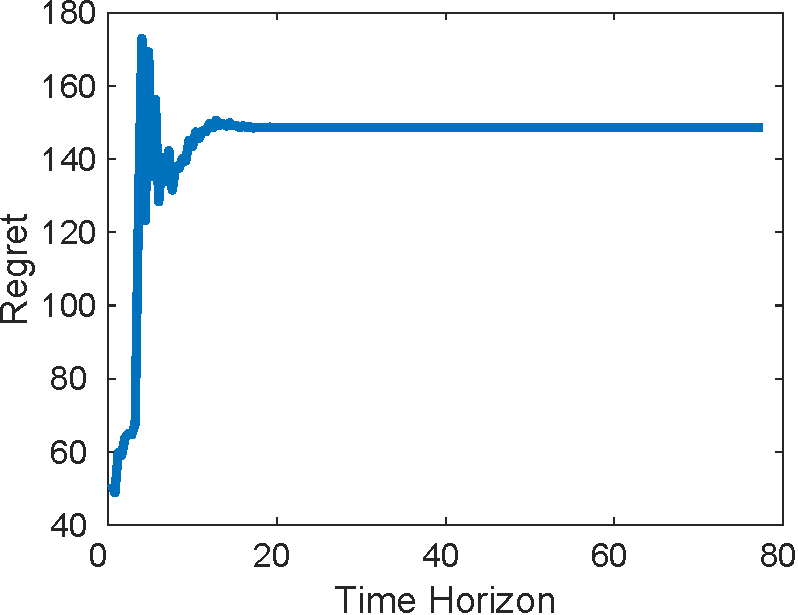
\includegraphics[width=.3\textwidth]{window2.pdf}
    \label{fig:ranSysReg}}
    \\
     \subfigure[Regret vs. Preview Window Length in 8-th Time Horizon]{
         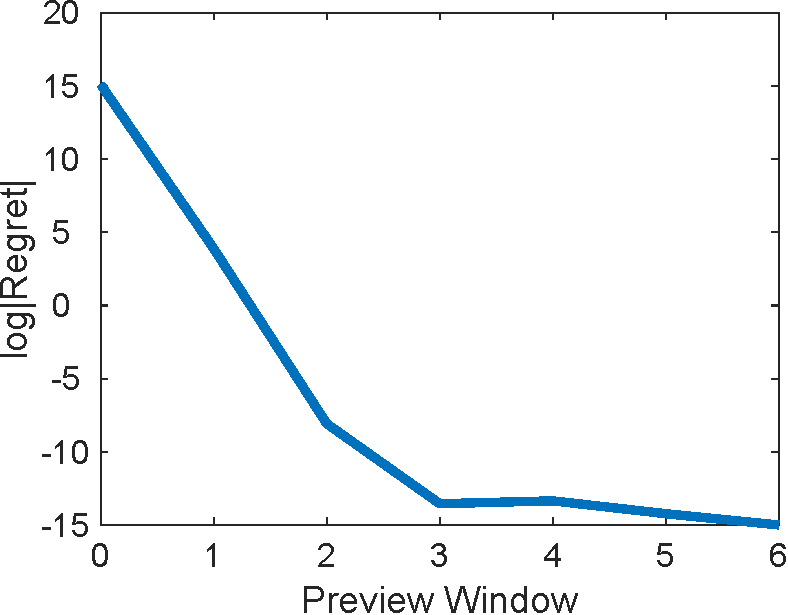
\includegraphics[width=.3\textwidth]{time1.pdf}
    \label{fig:PhysSysDisReg}}
     \subfigure[Regret vs. Preview Window Length in 69-th Time Horizon]{
         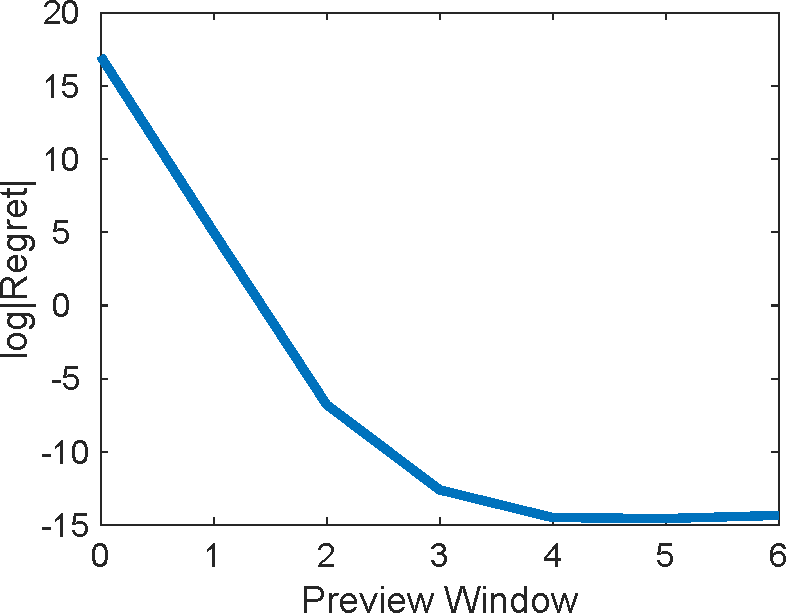
\includegraphics[width=.3\textwidth]{timeThird.pdf}
    \label{fig:RanSysDisReg}}
    \caption{Performance measure $\text{Regret}_{T}$ for simulated systems.}
\end{figure}

\section{CONCLUSIONS AND FUTURE WORKS}

%%%%%%%%%%%%%%%%%%%%%%%%%%%%%%%%%%%%%%%%%%%%%%%%%%%%%%%%%%%%%%%%%%%%%%%%%%%%%%%%
\section{ACKNOWLEDGMENTS}

The authors gratefully acknowledge the contribution of National Research Organization and reviewers' comments.


%%%%%%%%%%%%%%%%%%%%%%%%%%%%%%%%%%%%%%%%%%%%%%%%%%%%%%%%%%%%%%%%%%%%%%%%%%%%%%%%

References are important to the reader; therefore, each citation must be complete and correct. If at all possible, references should be commonly available publications.

\bibliographystyle{plain}
\bibliography{References}
\appendix
\end{document}
